\documentclass{beamer}

\mode<presentation> {
\usetheme{Madrid}
}

\usepackage{graphicx} % Allows including images
\usepackage{booktabs}
\usepackage{amsmath,amsthm,amssymb,amsfonts,extarrows}

%----------------------------------------------------------------------------------------
%	TITLE PAGE
%----------------------------------------------------------------------------------------

\title[MF796 - Computational Methods]{Deep Learning in Asset Pricing} % The short title appears at the bottom of every slide

\author{Present by: Haoyu Guan, Yanbin Liu, Chang Deng, Yuxuan Liu\\
Group 7 } % Your name
\institute[BU] % Your institution as it will appear on the bottom of every slide, may be shorthand to save space
{
MS in Mathematical Finance, Questrom \\ % Your institution for the title page
\medskip
Boston University
\medskip
}

\date{\today} % Date, can be changed to a custom date





\begin{document}
\begin{frame}
\titlepage % Print the title page as the first slide
\end{frame}

\begin{frame}
\frametitle{Overview}
\tableofcontents % Throughout your presentation, if you choose to use \section{} and \subsection{} commands, these will automatically be printed on this slide as an overview of your presentation
\end{frame}

%----------------------------------------------------------------------------------------
%	PRESENTATION SLIDES
%----------------------------------------------------------------------------------------

%------------------------------------------------
\section{Basic Conception} % Sections can be created in order to organize your presentation into discrete blocks, all sections and subsections are automatically printed in the table of contents as an overview of the talk
%------------------------------------------------

\subsection{Stochastic Discount Factor} % A subsection can be created just before a set of slides with a common theme to further break down your presentation into chunks

\begin{frame}
\frametitle{Basic Conception}
\begin{block}{Stochastic Discount Factor in Asset Pricing}
\begin{itemize}
\item What is the Stochastic Discount Factor(SDF)?
\item Implementation in finance area: By No-Arbitrage Pricing Theory, Stochastic Discount Factor(SDF) explains why the different expected returns come from different assets
\end{itemize}
\end{block}

\begin{block}{Challenges:}
\begin{itemize}
\item SDF includes all avaliable economic information
\item The function form of SDF is unknown and complicated
\item SDF needs to capture time-variation in economic conditions
\item Risk premium in stock return has a low signal-to-noise ratio
\end{itemize}
\end{block}
\end{frame}

%------------------------------------------------

\begin{frame}
\frametitle{Basic Conception}
\begin{block}{Goals of this project}
\begin{itemize}
\item Using deep neural networks to estimate SDF function, generate non-linear pricing model, and construct a optimal portfolio
\end{itemize}
\end{block}
\begin{block}{Contribution}
\begin{itemize}
\item Empirically outperforms all benchmark models
\item Optimal portfolio has out-of-sample Sharp ratio of XXXX
\item Take into account non-linearities and interaction between firm information
\item Most relevant firm characteristics are price trends, profitability, and capital structure variables.
\end{itemize}
\end{block}
\end{frame}

%------------------------------------------------
\section{Models}
\subsection{Neural Networks: SGD, LSTM, GAN}


\begin{frame}

\frametitle{Models}

\begin{itemize}
%\begin{math}
\item Fundamental no-arbitrage condition:\\
$$E\left[M_{t+1} R_{t+1, i}^{e} \hat{I}_{i, t}\right]=0$$

\item For a set of conditioning varibales$\hat{I}_{i,t} = \hat{g}(I_{t}, I_{i,t})$, the approach is to minimizes the corresponding loss function:

$$\min _{\omega} \max _{g} \frac{1}{N} \sum_{j=1}^{N}\left\|\mathbb{E}\left[\left(1-\sum_{i=1}^{N} \omega\left(I_{t}, I_{t, i}\right) R_{t+1, i}^{e}\right) R_{t+1, j}^{e} g\left(I_{t}, I_{t, j}\right)\right]\right\|^{2}$$

\item Create SDF network for the SDF $M_{t+1}$

\item Generate conditional network(FFN) for conditioning variableS$\hat{I}_{i,t}$

\item Implement Generative Adversarial Network(GAN) to minimize loss function
\end{itemize}


\end{frame}
%------------------------------------------------
\begin{frame}
Model Architecture:
\frametitle{Models}
\begin{figure}
    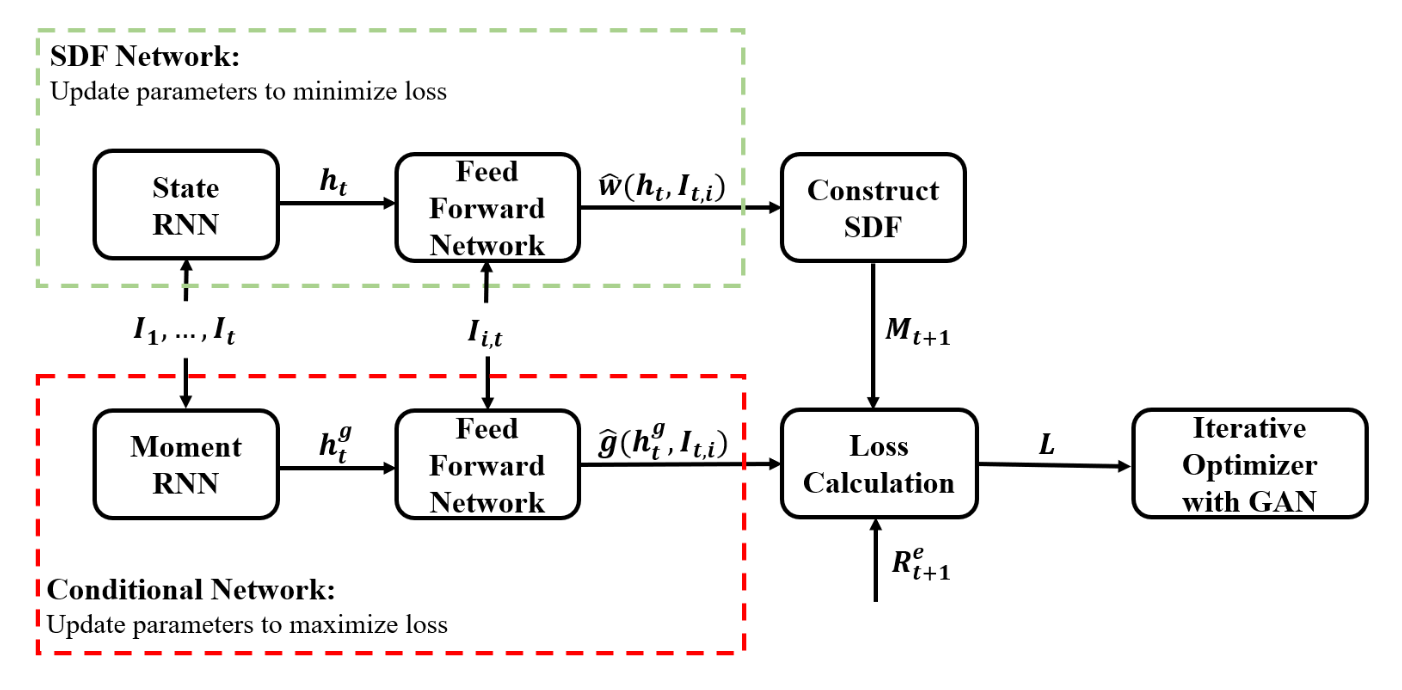
\includegraphics[width=12cm, hight=13cm]{model architecture.png}
\end{figure}
\end{frame}
%-------------------------------------------

\begin{frame}

\frametitle{Data}
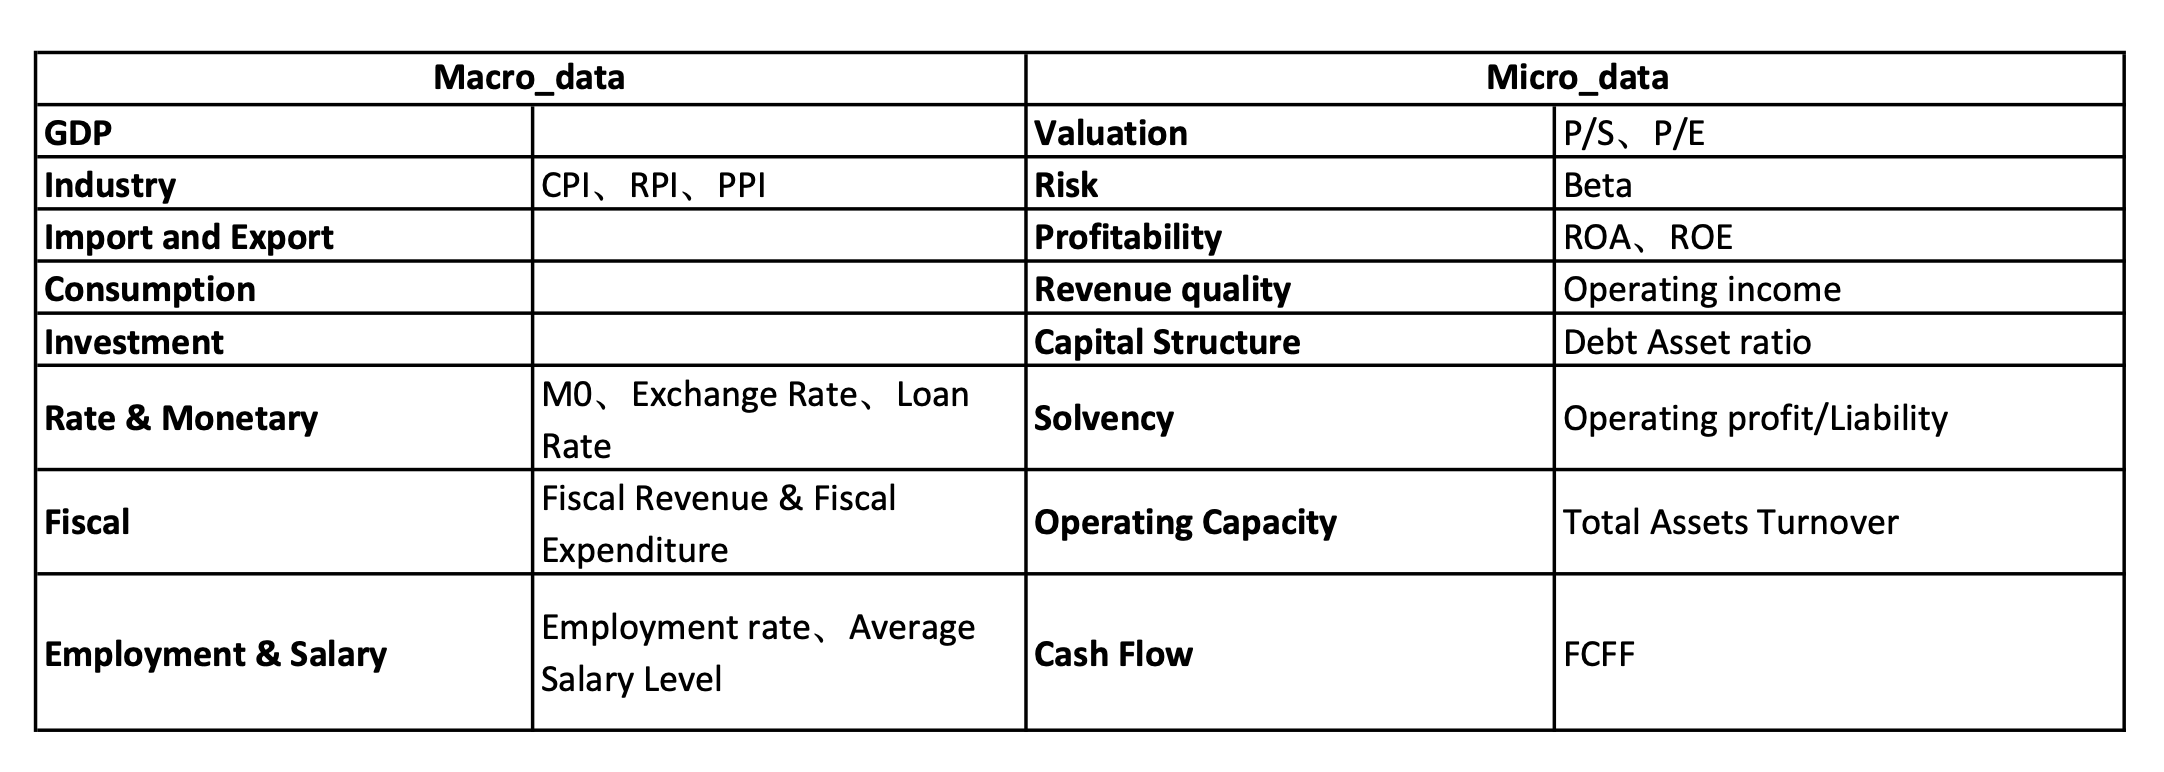
\includegraphics[width=12cm,height=5.5cm]{data_table.png}

From Wind database, acquire macroeconomic data and firm-specific data since 20070101 up to now. Re-sample and normalize to construct input for our model.


\end{frame}
%------------------------------------------------
\section{Backtesting Results}
%------------------------------------------------
\begin{frame}
\frametitle{Backtesting Results}
\begin{figure}
   \includegraphics[width=10cm,height=5cm]{loss.jpg}
\end{figure}

\end{frame}
%---------------------------------------------

\begin{frame}
\frametitle{Backtesting Results}
\begin{figure}
   \includegraphics[width=12cm,height=4.3cm]{train.jpg}
\end{figure}
\end{frame}

\begin{frame}
\frametitle{Backtesting Results}
\begin{figure}
   \includegraphics[width=12cm,height=4.3cm]{val.jpg}
\end{figure}
\end{frame}

\begin{frame}
\frametitle{Backtesting Results}
\begin{figure}
   \includegraphics[width=12cm,height=4.3cm]{test.jpg}
\end{figure}
\end{frame}
%------------------------------------------------

%------------------------------------------------

%------------------------------------------------

%------------------------------------------------
\begin{frame}
\frametitle{Backtesting Results}


\begin{table}
\begin{tabular}{cccc}
\toprule
& Train & Va1 & Testing \\
\midrule
\textbf{Benchmark} & 0.801714 & 1.354198 & 0.080040 \\
\textbf{MV} & 1.336177 & 1.929056 & -0.093803 \\
\textbf{GAN} & 1.801015 & 2.458797 & 0.15558 \\
\bottomrule
\end{tabular}
\caption{Result}
\end{table}


\end{frame}

%------------------------------------------------

\begin{frame}
\frametitle{References}
\footnotesize{
\begin{thebibliography}{99} % Beamer does not support BibTeX so references must be inserted manually as below
\bibitem[Smith, 2012]{p1} Luyang Chen,  Markus Pelger, Jason Zhu (2019)
\newblock Deep Learning in Asset Pricing(December 4, 2019), Stanford University
\newblock \emph{ Available at SSRN: https://ssrn.com/abstract=3350138 or http://dx.doi.org/10.2139/ssrn.3350138
}
\end{thebibliography}
}
\end{frame}

%------------------------------------------------

\begin{frame}
\frametitle{Conclusion}
\Huge{\centerline{Thanks for listening}}
\end{frame}

%--------------------------------------------------------------

\end{document}
